\documentclass[a4paper]{article}

%% Language and font encodings
\usepackage[brazil]{babel}
\usepackage[utf8x]{inputenc}
\usepackage[T1]{fontenc}

%% Sets page size and margins
\usepackage[a4paper,top=3cm,bottom=2cm,left=3cm,right=3cm,marginparwidth=1.75cm]{geometry}

%% Useful packages
\usepackage{amsmath}
\usepackage{graphicx}
\usepackage[colorinlistoftodos]{todonotes}
\usepackage[colorlinks=true, allcolors=blue]{hyperref}
\usepackage{ragged2e}
\usepackage{setspace}
\usepackage{enumitem}
\usepackage{float}
\usepackage{caption}
% \usepackage{biblatex}

\newcommand*{\Scale}[2][4]{\scalebox{#1}{$#2$}}%
\newcommand*{\Resize}[2]{\resizebox{#1}{!}{$#2$}}%

\title{Tubo de Pitot no túnel de vento}
\author{Nikolas Bernardes Vieira de Freitas}

\setlength{\parindent}{2em}
\renewcommand{\baselinestretch}{1.5}

\begin{document}
\maketitle

\section{Resumo}
    O experimento sobre o túnel de vento tem como objetivo demonstrar a diminuição da pressão estática, com a medição sendo feita por uma sonda de pressão. Conectou-se a sonda ao túnel de vento para medição da pressão estática, e conforme o diâmentro deste túnel diminui, a velocidade aumenta e o óleo contido na sonda se desloca para esquerda e para cima devido ao a diminuição da pressão estática $p_{est}$ contida naquele lado da sonda. Notamos que o experimento cumpre seu objetivo quando observa-se os gráficos de altura do fluído e de pressão estática.

\section{Introdução}
      Os fluídos quando estão expostos a uma aceleração gravitacional $g$ tendem a ficar o mais próximo possível da origem desta aceleração. Quando um fluído de maior densidade se mantém no ponto mais próximo da origem desta aceleração e, se houver outro fluído de menor densidade afetado pela mesma aceleração, o de maior densidade aplica uma força de mesma direção e sentido contrário à força do fluído de menor densidade que acaba por ficar sob o mesmo, assim mantendo um equilibrio estático dentre os fluídos. Isto explica a base do funcionamento da sonda de pressão.

     Segundo o princípio de Bernoulli um fluído na horizonntal, quanto maior a velocidade deste fluído menor é a pressão exercida pelo mesmo. O lado do duto da sonda de pressão que está dentro do túnel de vento vai ter a pressão atmosférica $p_a$ reduzida, logo o fluído dentro da sonda de pressão se moverá verticalmente na direção do túnel de vento. E quanto mais estreito for túnel de vento, maior a velocidade do ar em relação a sonda de pressão, logo menor pressão estática $p_{est}$.

\section{Materiais}
    \begin{enumerate}[label=(\roman*)]
        \item Sonda de pressão
        \item Túnel de vento
    \end{enumerate}

\section{Montagem}
    Acopla-se a sonda de pressão no túnel de vento de diâmetro variável. Um dos dutos da sonda ficou descoberto para aplicar a pressão atmosférica e o outro duto ficou dentro do túnel de vento.

\section{Procedimento}

\section{Dados obtidos}
    Os dados obtidos durante o funcionamento do túnel de vento
    \begin{center}
          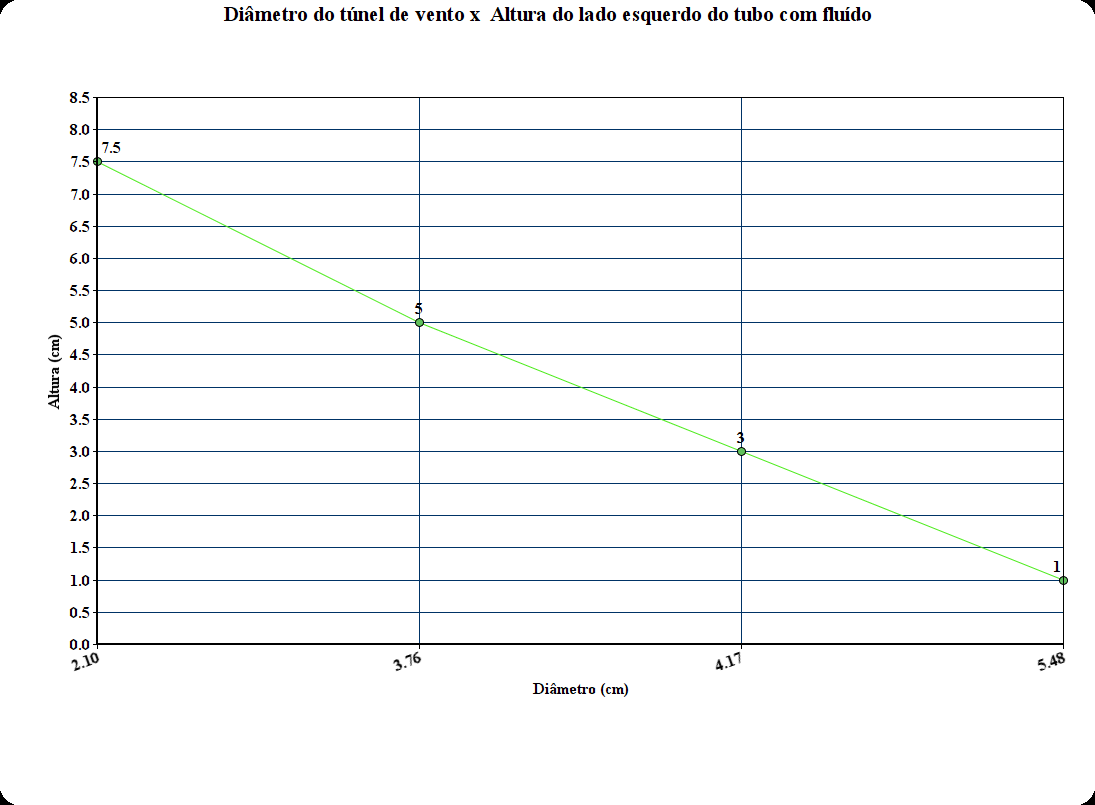
\includegraphics[width=\linewidth]{img/graphHeight.png}
          \label{graph}{gráfico: 1}
    \end{center}


\section{Discussão dos dados}
    Segue as pressões estáticas $p_{est}$ calculadas para cada diâmetro do túnel de vento.
        \begin{center}
              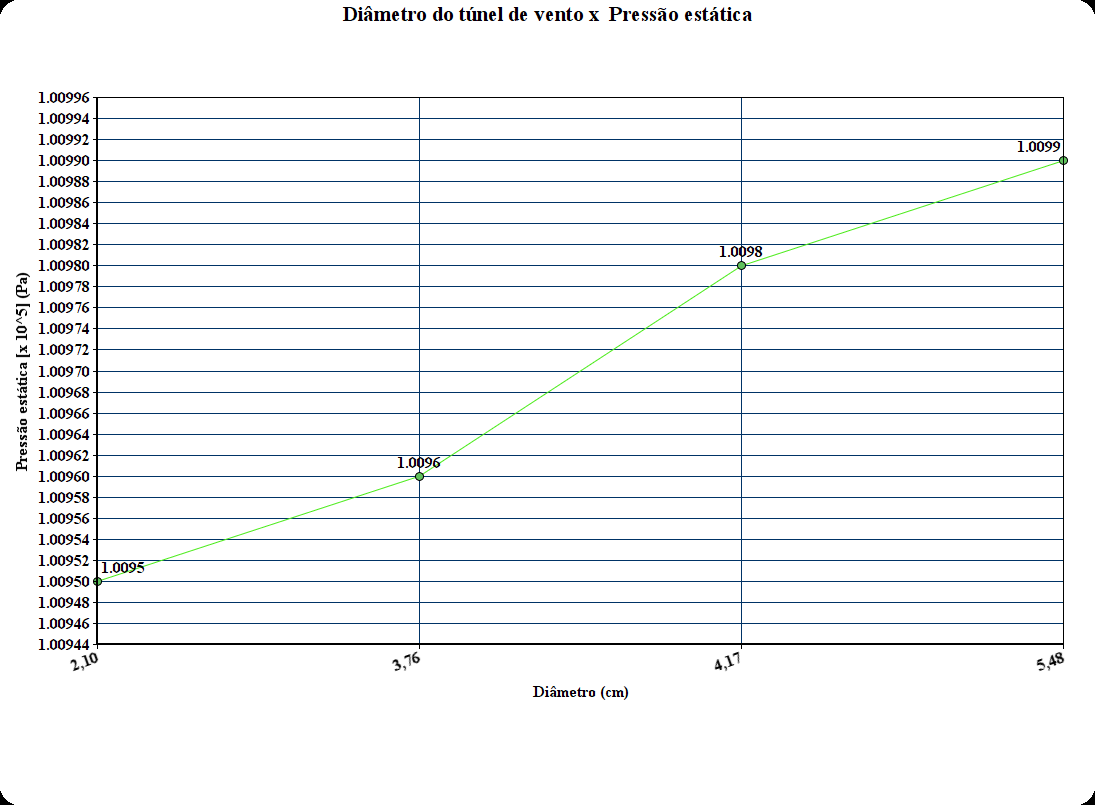
\includegraphics[width=\linewidth]{img/graphPression.png}
              \label{graph}{gráfico: 2}
        \end{center}

        Como pôde-se ver no gráfico de medidas obtidas pela observação \textit{[gráfico: 1]}, o crescimento da altura não é totalmente linear. Isso deve-se ao fato de que o fluído real não se comporta exatamente como um fluído ideal. No fluído real temos problema de inércia, compressão e viscodisade, o que influi nas medidas. As pressões resultantes acompanham esse comportamento como se pode ver no gráfico sobre de pressão estática \textit{[gráfico: 2]}.

\section{Conclusão}

\begin{thebibliography}{1}

\bibitem{knuthwebsite}
    Wikipedia: Lei da queda dos corpos,
    \\\texttt{https://pt.wikipedia.org/wiki/Lei\_da\_queda\_dos\_corpos}
\end{thebibliography}

\end{document}
